\documentclass[11pt,a4paper]{article}

\usepackage[T1]{fontenc}
\usepackage[utf8]{inputenc}
\usepackage{newtxtext,newtxmath}
\usepackage[a4paper,margin=2.5cm]{geometry}
\usepackage{amsmath}
\usepackage{booktabs}
\usepackage{tabularx}
\usepackage{array}
\usepackage{enumitem}
\usepackage{microtype}
\usepackage{xcolor}
\usepackage{pgfplots}
\usepackage[font=small,labelfont=bf]{caption}
\usepackage[colorlinks=true,linkcolor=black,citecolor=black,urlcolor=blue!50!black]{hyperref}

\pgfplotsset{compat=1.18}
\definecolor{refdefault}{HTML}{DEDED8}
\definecolor{refactive}{HTML}{BDBDB0}
\definecolor{fastblue}{HTML}{2A78D6}

\newcommand{\DJF}{DJTLED\_fast}
\newcommand{\code}[1]{\texttt{#1}}
\newcommand{\Jm}{J^{-2/3}}
\newcommand{\mat}[1]{\mathbf{#1}}
\newcolumntype{Y}{>{\raggedright\arraybackslash}X}
\setlist{itemsep=2pt,topsep=4pt}
\setlength{\parskip}{6pt plus 1pt}
\setlength{\parindent}{0pt}

\title{\textbf{A Faster DJ-TLED: Data-Layout and Arithmetic Optimisations of a Direct-Jacobian Explicit Finite Element Solver on CPU}}
\author{Baiqi Cheng}
\date{18 November 2026}

\begin{document}
\maketitle

\begin{abstract}
\noindent
DJ-TLED is a total Lagrangian explicit dynamics finite element algorithm that computes nodal forces from the element Jacobian alone. This paper keeps the algorithm unchanged and asks how much faster its CPU implementation can be made. A second implementation, \DJF, stores each element in 88 bytes instead of 448, evaluates eight elements at a time with SIMD instructions, removes nine of ten divisions from the force expression, replaces the power function for $\Jm$ by a warm-started Newton iteration, keeps one thread team for the whole run, and renumbers the mesh for memory locality. Both implementations were measured on two neo-Hookean tension models of 6,713 and 361,175 tetrahedra, with 1 to 10 threads on a processor with 4 performance and 6 efficiency cores, under equal thread counts and wait policies. \DJF{} was 2.1 to 2.7 times faster on the small model and 2.5 to 7.1 times faster on the large one. The final displacements of the two implementations differ by 0.0016\,\% and 0.042\,\% of the prescribed displacement, which equals the distance of either from the reference results, and are identical for every thread count. A time-step sweep shows that single-precision rounding, not the time step, limits agreement on the large model to about 0.3\,\%.
\end{abstract}

%======================================================================
\section{Introduction}
\label{sec:intro}

The DJ-TLED algorithm can run several times faster on a CPU without any change to its formulation. This paper shows how, and measures the gain against the reference implementation.

\subsection{Background}

Interactive applications such as surgical simulation and image-guided surgery need nonlinear finite element solutions of soft-tissue deformation in real time. The total Lagrangian explicit dynamics (TLED) algorithm \cite{miller2007} is the usual starting point. It refers all quantities to the undeformed configuration, so spatial derivatives are computed once. It integrates in time with the explicit central-difference scheme and a lumped mass matrix, so no system of equations is assembled or solved. It uses low-order elements, so the work per element is small. Every operation is local to an element or a node, which suits parallel hardware \cite{taylor2008}.

DJ-TLED \cite{zhang2021} reformulates TLED so that the nodal forces of an element are written in terms of the Jacobian operator alone. The deformation gradient, the right Cauchy--Green tensor and the second Piola--Kirchhoff stress are never formed. The quantities that do not change in time are collected into precomputed tensors, and only the element Jacobian is updated at run time. Zhang \cite{zhang2021} reports CPU solution times between 0.70 and 0.88 of those of TLED, and GPU speed-ups of up to 121.72 for tetrahedral meshes. A reference implementation in C++ with OpenMP, for 4-node tetrahedra and a neo-Hookean material, is published with the paper \cite{djtledcode}.

\subsection{The question studied here}

DJ-TLED reduced the number of operations in the formulation. This paper asks a narrower question: with the formulation fixed, how much time does the CPU implementation still leave unused?

The question matters because an explicit solver repeats one small kernel a very large number of times. The larger test model in this paper has 361,175 elements and runs 40,000 steps, which is $1.4\times10^{10}$ element force evaluations. The run time is therefore set by the cost of one evaluation and by the fixed overhead of one step. Both depend on how the data is laid out in memory, on how many expensive arithmetic operations the kernel performs, and on how the threads are coordinated. None of them depends on the formulation.

\subsection{Where the reference implementation can be improved}

A reading of the reference code \cite{djtledcode} gives five places where time is lost or robustness can be gained (Table~\ref{tab:areas}).

\begin{table}[ht]
\centering
\small
\caption{Where the reference implementation can be improved.}
\label{tab:areas}
\begin{tabularx}{\linewidth}{@{}l Y Y@{}}
\toprule
Area & Reference implementation & Consequence \\
\midrule
Element data & One heap object of 448 bytes per element, reached through a pointer. It holds data used only during set-up, such as six $3\times3$ matrices. & Each force evaluation pulls in memory it does not need, and the scattered objects prevent vectorisation. \\
\addlinespace
Arithmetic & A full $3\times3$ inverse with nine divisions, one call to \code{powf} for $\Jm$, and two precomputed arrays that carry the same information. & Divisions and \code{powf} are the slowest operations in the kernel. \\
\addlinespace
Threading & A new parallel region every step. Thread $k$ takes elements $k$, $k+T$, $k+2T$ and so on. All cores are used equally. & Thread start-up is paid every step, every thread sweeps the whole mesh, and slow cores hold back fast ones. \\
\addlinespace
Numbering & Elements and nodes are processed in input order. & Speed depends on how the mesh generator numbered the mesh. \\
\addlinespace
Robustness & An inverted element is noticed only when it produces a not-a-number. & A failure is reported late and without its cause. \\
\bottomrule
\end{tabularx}
\end{table}

\subsection{Contribution}

This paper presents \DJF, a second implementation of the same algorithm with the same input format, the same single-precision arithmetic and the same boundary-condition rules. It makes seven changes, each described with its mathematics and rationale in Section~\ref{sec:method}:
\begin{enumerate}
\item a compact element record stored in blocks of eight and evaluated with SIMD instructions;
\item an algebraic simplification of the nodal force that removes one precomputed array and eight of the nine divisions;
\item a warm-started Newton iteration for $\Jm$ in place of \code{powf};
\item one thread team for the whole run, with spinning instead of sleeping between phases;
\item one thread per performance core on processors with two kinds of core;
\item reverse Cuthill--McKee renumbering of nodes and elements;
\item an explicit check for inverted elements.
\end{enumerate}
Section~\ref{sec:results} compares the two implementations on two models across CPU configurations of 1 to 10 threads, in speed and in accuracy. Section~\ref{sec:conclusion} concludes.

%======================================================================
\section{Methodology}
\label{sec:method}

Both solvers compute exactly the formulation of Zhang \cite{zhang2021} summarised in Section~\ref{sec:formulation}. Sections~\ref{sec:blocks} to~\ref{sec:inverted} describe what \DJF{} does differently, and Section~\ref{sec:unchanged} lists what it deliberately keeps.

\subsection{The DJ-TLED formulation used by both solvers}
\label{sec:formulation}

\textbf{Kinematics.} Consider a 4-node tetrahedron. Let $\mat{X}_e$ and $\mat{U}_e$ be the $3\times4$ matrices whose columns are the initial coordinates and the current displacements of its nodes. The derivatives of the linear interpolation functions with respect to the natural coordinates are constant:
\begin{equation}
\mat{H}_{\xi} = \begin{bmatrix} -1 & 1 & 0 & 0 \\ -1 & 0 & 1 & 0 \\ -1 & 0 & 0 & 1 \end{bmatrix}.
\end{equation}
The Jacobian operator at time $0$ is computed once, and at time $t$ it is obtained by adding displacement differences (Eq.~11 of \cite{zhang2021}). Row $i$ of $\mat{J}_t$ is the edge vector from node 1 to node $i+1$.
\begin{equation}
\mat{J}_0 = \mat{H}_{\xi}\,\mat{X}_e^{T}, \qquad \mat{J}_t = \mat{J}_0 + \mat{H}_{\xi}\,\mat{U}_e^{T}.
\end{equation}
The volume ratio follows from two determinants (Eq.~12 of \cite{zhang2021}), and the initial volume of the element is $V_0 = \det(\mat{J}_0)/6$.
\begin{equation}
J = \frac{\det \mat{J}_t}{\det \mat{J}_0}.
\end{equation}

\textbf{Material.} The neo-Hookean strain energy is used in its uncoupled form, with shear modulus $\mu$ and bulk modulus $\kappa$. Here $I_1$ is the first invariant of the right Cauchy--Green tensor $\mat{C}$.
\begin{equation}
\Psi = \frac{\mu}{2}\left(\bar{I}_1 - 3\right) + \frac{\kappa}{2}\left(J - 1\right)^2, \qquad \bar{I}_1 = \Jm\, I_1, \qquad I_1 = \operatorname{tr}\mat{C}.
\end{equation}

\textbf{Nodal forces.} Substituting this energy into the direct Jacobian force expression (Eq.~10 of \cite{zhang2021}) gives the $3\times4$ matrix of nodal forces of one element. Column $a$ is the force on node $a$.
\begin{equation}
\label{eq:force}
\mat{F}_e = \left[ \Jm\,\frac{\mu}{2}\,\mat{J}_t^{T}\,\mat{I}_{1m} + \left( -\frac{\mu}{3}\,\Jm\,I_1 + \kappa\,J\,(J-1) \right) V_0\,\mat{J}_t^{-1} \right] \mat{H}_{\xi}.
\end{equation}
The tensor $\mat{I}_{1m}$ is constant in time and is precomputed (Eq.~37 of \cite{zhang2021}).
\begin{equation}
\mat{I}_{1m} = 2\,V_0\,\mat{J}_0^{-T}\,\mat{J}_0^{-1}.
\end{equation}
The invariant $I_1$ is obtained without forming $\mat{C}$. With $\mat{g} = \mat{J}_t\mat{J}_t^{T}$, its six distinct components are collected in a vector and multiplied by a precomputed vector $\mat{m}_1$ (Eqs.~17, 18, 23 and 27 of \cite{zhang2021}). The entries of $\mat{m}_1$ are the traces of six constant matrices $\mat{G}_{ij}$.
\begin{equation}
\label{eq:I1}
I_1 = \hat{\mat{g}}^{T}\,\mat{m}_1, \qquad \hat{\mat{g}} = \left[\, g_{11}\;\; g_{22}\;\; g_{33}\;\; g_{12}\;\; g_{13}\;\; g_{23} \,\right]^{T}.
\end{equation}
Because of the structure of $\mat{H}_{\xi}$, columns 2 to 4 of $\mat{F}_e$ are the three columns of the bracketed matrix, and column 1 is minus their sum. Nine force components are computed and three follow by subtraction.

\textbf{Time integration.} With a lumped mass matrix $\mat{M}$ and mass-proportional damping $\mat{D} = \alpha\mat{M}$, the equation of motion (Eq.~13 of \cite{zhang2021}) is uncoupled per degree of freedom. For a degree of freedom with nodal mass $m$, internal force $f$ and external force $r$, the central-difference update is
\begin{equation}
\label{eq:update}
u^{n+1} = c_1\,(r - f^{\,n}) + c_2\,u^{n} + c_3\,u^{n-1},
\end{equation}
\begin{equation}
c_1 = \left( \frac{m}{\Delta t^2} + \frac{\alpha\,m}{2\,\Delta t} \right)^{-1}, \qquad c_2 = \frac{2\,m\,c_1}{\Delta t^2}, \qquad c_3 = \frac{\alpha\,m\,c_1}{2\,\Delta t} - \frac{c_2}{2}.
\end{equation}
Each node receives a quarter of the mass $\rho V_0$ of every element it belongs to. A prescribed displacement is ramped linearly over the total time, a fixed degree of freedom is set to zero, and gravity enters as an external force.

\textbf{Stability.} The scheme is conditionally stable. The time step is bounded by the smallest characteristic element length $L_e$ and the dilatational wave speed $c$ (Eq.~14 of \cite{zhang2021}).
\begin{equation}
\label{eq:stability}
\Delta t \le \frac{L_e}{c}, \qquad c = \sqrt{\frac{\kappa + \tfrac{4}{3}\mu}{\rho}}.
\end{equation}

\textbf{One time step.} Both solvers execute a step in two passes, with all threads synchronised between them:
\begin{enumerate}
\item Element pass. Every element computes $\mat{F}_e$ from the current displacements and writes its 12 components into a buffer slot that belongs to that element alone.
\item Node pass. Every node sums the force components of the elements around it, using a precomputed list, and applies the update of Eq.~\eqref{eq:update} to its three degrees of freedom.
\end{enumerate}
No two threads ever write the same memory, so no locks are needed. This two-pass structure comes from the reference implementation and is kept. The cost of a step is therefore $N_e$ kernel evaluations plus $N_n$ node updates, each of which gathers about $4N_e/N_n$ force triples. That ratio is 18.6 for the small test model and 21.4 for the large one.

\subsection{Compact element blocks and SIMD evaluation}
\label{sec:blocks}

\textbf{Change.} Each element is reduced to the 21 numbers the force kernel reads, and elements are stored in blocks of $W = 8$ so that one kernel call evaluates eight elements with SIMD instructions.

\textbf{What the kernel needs.} Per element: four node indices, the nine entries of $\mat{J}_0$, the six distinct entries of a symmetric tensor $\mat{P}$ defined in Section~\ref{sec:algebra}, the reciprocal of $\det(\mat{J}_0)$, and the product $\kappa V_0$. That is 21 values, or 84 bytes.

\textbf{Layout.} The reference stores an array of structures: one object per element, allocated separately. The fast solver stores an array of structures of arrays. A block holds each of the 21 fields as an array of eight values, one per element, so the same field of eight elements is contiguous and loads as one vector (Table~\ref{tab:layout}).

\begin{table}[ht]
\centering
\small
\caption{Element storage in the two implementations.}
\label{tab:layout}
\begin{tabularx}{\linewidth}{@{}l Y Y@{}}
\toprule
 & Reference & \DJF \\
\midrule
Element record & 448-byte heap object, plus a separately allocated array for the material constants & 88 bytes, inside a 704-byte block of eight \\
Element force buffer & 48 bytes & 48 bytes \\
Reached by & pointer per element & index into a contiguous array \\
Evaluated & one element at a time & eight elements at a time \\
\bottomrule
\end{tabularx}
\end{table}

The sizes are those reported by the compiler for the two codes. The 448-byte object spans seven 64-byte cache lines. It includes six $3\times3$ matrices and other fields that are only needed during set-up.

\textbf{Kernel.} For one block the kernel first gathers the displacements of the $4\times8$ nodes into a local $12\times8$ array. It then runs the arithmetic of Section~\ref{sec:algebra} as a loop over the eight lanes, marked for vectorisation. It finally stores the $12\times8$ force components contiguously. The last block of a mesh is padded with inert elements, for which $\mat{J}_0$ is the identity and $\mat{P}$ and $\kappa V_0$ are zero. They produce $J = 1$ and zero force, so they need no special handling.

\textbf{Rationale.} An explicit solver has two regimes. A small mesh fits in cache and is limited by arithmetic, where SIMD helps directly. A large mesh is limited by the rate at which element data can be read from memory, where the fivefold smaller record helps. The block layout addresses both with one data structure. The width $W$ is a compile-time constant; Section~\ref{sec:contrib} reports widths 1, 4, 8 and 16.

\subsection{Algebraic simplification of the nodal force}
\label{sec:algebra}

\textbf{Change.} The force of Eq.~\eqref{eq:force} is rearranged so that one precomputed tensor replaces two precomputed arrays, and one division replaces ten.

\textbf{One tensor instead of two arrays.} Define the symmetric tensor
\begin{equation}
\mat{P} = \frac{\mu}{2}\,\mat{I}_{1m} = \mu\,V_0\,\mat{J}_0^{-T}\,\mat{J}_0^{-1}.
\end{equation}
The first term of the force is then $\Jm\,\mat{J}_t^{T}\mat{P}$. The invariant $I_1$ can be read from the same tensor. Since $\mat{C} = \mat{J}_0^{-1}\mat{J}_t\mat{J}_t^{T}\mat{J}_0^{-T}$, the cyclic property of the trace gives
\begin{equation}
I_1 = \operatorname{tr}\!\left( \mat{J}_0^{-1}\,\mat{J}_t\,\mat{J}_t^{T}\,\mat{J}_0^{-T} \right) = \operatorname{tr}\!\left( \mat{J}_0^{-T}\,\mat{J}_0^{-1}\,\mat{g} \right) \quad\Longrightarrow\quad \mu\,V_0\,I_1 = \mat{P} : \mat{g}.
\end{equation}
This is the same number as the product of $\hat{\mat{g}}$ with $\mat{m}_1$ in Eq.~\eqref{eq:I1}, because the entries of $\mat{m}_1$ are the entries of $\mat{J}_0^{-T}\mat{J}_0^{-1}$, with the off-diagonal ones doubled. The vector $\mat{m}_1$ therefore does not need to be stored. With the symmetry of $\mat{P}$ and $\mat{g}$, the double contraction costs six multiplications:
\begin{equation}
\mat{P} : \mat{g} = P_{11}g_{11} + P_{22}g_{22} + P_{33}g_{33} + 2\left( P_{12}g_{12} + P_{13}g_{13} + P_{23}g_{23} \right).
\end{equation}

\textbf{One division instead of ten.} The reference forms the full inverse of $\mat{J}_t$, dividing each of its nine cofactors by $\det(\mat{J}_t)$, and divides once more by $\det(\mat{J}_0)$ to obtain $J$. The force, however, only needs the inverse multiplied by a scalar. Writing the inverse as the adjugate over the determinant, the scalar and the determinant are combined first:
\begin{equation}
\label{eq:s}
s = \frac{ -\tfrac{1}{3}\,\Jm\,(\mat{P} : \mat{g}) + \kappa V_0\,J\,(J-1) }{ \det \mat{J}_t }, \qquad J = \det \mat{J}_t \cdot \frac{1}{\det \mat{J}_0},
\end{equation}
\begin{equation}
\label{eq:fastforce}
\mat{F}_e = \left[ \Jm\,\mat{J}_t^{T}\,\mat{P} + s\,\operatorname{adj}(\mat{J}_t) \right] \mat{H}_{\xi}.
\end{equation}
This is algebraically identical to the force of Eq.~\eqref{eq:force}. The reciprocal of $\det(\mat{J}_0)$ is stored, so the only division left per element is the one in $s$.

\textbf{Precomputation in double precision.} The constants $\mat{J}_0$, $\mat{P}$, $1/\det(\mat{J}_0)$ and $\kappa V_0$ are computed once in double precision and then rounded to single precision. The reference computes them in single precision. This costs nothing at run time and removes one source of rounding error from every step.

\textbf{Rationale.} Division is several times slower than multiplication and limits the throughput of a SIMD loop. Removing nine of ten divisions and one stored array reduces both the arithmetic and the memory read per element.

\subsection{Warm-started Newton iteration for \texorpdfstring{$\Jm$}{J\textasciicircum(-2/3)}}
\label{sec:newton}

\textbf{Change.} The call to \code{powf} in every element evaluation is replaced by two Newton iterations that start from the value the same element had in the previous step.

\textbf{Iteration.} The value $y = \Jm$ is the positive root of $f(y) = y^{-3} - J^2$. Newton's method for this function contains no division and no root:
\begin{equation}
\label{eq:newton}
y \leftarrow y - \frac{f(y)}{f'(y)} = \frac{y\left( 4 - J^2 y^3 \right)}{3}.
\end{equation}

\textbf{Convergence.} Write the current iterate as the exact value $y^{*}$ times $(1 + e)$. Then $J^2 y^3 = (1 + e)^3$, and one iteration gives
\begin{equation}
y_{\text{new}} = y^{*}\,(1+e)\left( 1 - e - e^2 - \tfrac{1}{3}e^3 \right) = y^{*}\left( 1 - 2e^2 + O(e^3) \right).
\end{equation}
The relative error is squared and doubled at each iteration.

\textbf{Starting value and acceptance test.} Under the stability limit of Eq.~\eqref{eq:stability} an element deforms very little in one step, so its previous $\Jm$ is an excellent starting value. One 4-byte value is stored per element. Before iterating, the kernel evaluates $r = J^2 y^3$ and accepts the warm start only if $|r - 1| < 10^{-2}$. This bounds the starting error by $|e| < 3.4\times10^{-3}$. Two iterations then reduce it to about $2.3\times10^{-5}$ and $1.0\times10^{-9}$, which is below the single-precision rounding unit of $6\times10^{-8}$. The result is therefore correct to rounding.

\textbf{Fallback.} If the test fails for an element, that element alone is recomputed with \code{powf}. In every run reported in this paper the number of fallbacks was zero.

\textbf{Rationale.} \code{powf} is a library call that the compiler cannot vectorise, so it would force the eight-lane loop of Section~\ref{sec:blocks} to process one element at a time. The iteration is five multiplications and one subtraction per pass and vectorises fully.

\subsection{One thread team and spin waiting}
\label{sec:threads}

\textbf{Change.} The threads are created once, before the time loop, and wait actively between the two passes of a step.

\textbf{Mechanism.} The reference opens a parallel region in every step, which hands work to the threads and collects them again 40,000 times in the larger test. The fast solver opens one parallel region around the whole time loop. Every thread runs the loop itself and keeps its own copy of the three pointers to the previous, current and next displacement arrays, which it rotates after each step. The element pass and the node pass are work-sharing loops inside that region, and file output runs on a single thread. Waiting threads spin instead of sleeping. This active wait policy is a setting of the OpenMP runtime, not a property of the algorithm, and the reference can be given it as well; Section~\ref{sec:results} measures the reference both ways.

\textbf{Contiguous shares.} The reference gives thread $k$ the elements $k$, $k+T$, $k+2T$ and so on. Every thread therefore walks the whole mesh, and neighbouring elements are handled by different threads. The 48-byte force record of an element then shares a 64-byte cache line with a record that another thread writes. The fast solver gives each thread one contiguous range of blocks and of nodes, so each thread works on its own region of memory.

\textbf{Rationale.} A step of the small model takes about 20 microseconds. Waking a sleeping thread takes a comparable time, so with sleeping threads the synchronisation costs as much as the computation. Spinning removes that delay. The cost is that a spinning thread occupies its core, which Section~\ref{sec:contrib} shows is harmful when the machine is busy with other work.

\subsection{One thread per performance core}
\label{sec:pcores}

\textbf{Change.} On processors with performance and efficiency cores, the default thread count is the number of performance cores.

\textbf{Rationale.} With equal shares of work per thread, a step ends when the slowest thread ends. An efficiency core that is several times slower than a performance core therefore sets the pace for all of them. The count can be overridden; Section~\ref{sec:speed} measures 1 to 10 threads for both solvers.

\subsection{Renumbering of nodes and elements}
\label{sec:renumber}

\textbf{Change.} Before the time loop, nodes are renumbered by the reverse Cuthill--McKee algorithm \cite{cuthill1969} and elements are sorted by their lowest and highest node number. Results are written in the original numbering.

\textbf{Mechanism.} Two nodes are adjacent if they share an element. Reverse Cuthill--McKee orders the nodes by a breadth-first traversal from a peripheral node, which keeps adjacent nodes close in number. The four nodes of an element then lie close together in the displacement array, and the elements around a node lie close together in the force buffer.

\textbf{Rationale.} Both passes gather data by index: the element pass gathers displacements and the node pass gathers forces. If the indices of neighbours are far apart, every gather is a cache miss. The benefit depends on how the mesh generator numbered the input, so it varies from model to model. The renumbering is done once, before the timed loop; it added about 1\,ms to the preparation of the small model and about 65\,ms to that of the large one.

\subsection{Detection of inverted elements}
\label{sec:inverted}

\textbf{Change.} The solver checks that $\det(\mat{J}_0)$ is positive for every element of the input mesh, and that $J$ is positive for every element at every step.

\textbf{Rationale.} A volume ratio $J$ of zero or less means an element has collapsed or turned inside out, which is physically inadmissible and usually signals a time step above the stability limit. The reference notices this only indirectly, when \code{powf} of a negative number returns a not-a-number that later reaches a displacement. The iteration of Section~\ref{sec:newton} works with $J^2$ and so cannot see the sign of $J$ at all. The explicit test closes that gap and reports the cause and the step at which it occurred.

\subsection{What is deliberately unchanged}
\label{sec:unchanged}

\begin{itemize}
\item \textbf{Single precision.} Both solvers compute and store displacements and forces as 32-bit floats.
\item \textbf{The two-pass step and the fixed summation order.} Each node sums the forces of its elements in a fixed order, so the result does not depend on the number of threads or on how the loops are scheduled.
\item \textbf{The integration constants and boundary-condition rules} of Section~\ref{sec:formulation}.
\end{itemize}
The two solvers can therefore differ only through rounding: the rearranged kernel, the Newton iteration, the double-precision constants and the order in which forces are summed at a node. Section~\ref{sec:accuracy} measures how large that difference is.

%======================================================================
\section{Results}
\label{sec:results}

\subsection{Test set-up}
\label{sec:setup}

Both solvers were run on the same two models, on one machine, under the same run conditions.

\textbf{Models.} Both are a cube of side 0.1 with one face displaced by 0.05 in $y$, ramped linearly over a total time of 1, and the opposite face fixed. The material is neo-Hookean with $\mu = 6{,}567$, $\kappa = 326{,}210$, density 1,060 and damping coefficient $\alpha = 5$, in the units of the model files. A reference displacement field is distributed with each model and is used only in Section~\ref{sec:accuracy}. Table~\ref{tab:models} gives their sizes.

\begin{table}[ht]
\centering
\small
\caption{The two test models.}
\label{tab:models}
\begin{tabular}{@{}lrr@{}}
\toprule
 & Small model & Large model \\
\midrule
Nodes & 1,440 & 67,362 \\
Elements & 6,713 & 361,175 \\
Time step & 0.00025 & 0.000025 \\
Steps & 4,000 & 40,000 \\
Element evaluations in a run & $2.7\times10^{7}$ & $1.4\times10^{10}$ \\
\bottomrule
\end{tabular}
\end{table}

\textbf{Machine and build.} Apple M5 with 4 performance cores and 6 efficiency cores, 24\,GB of memory, no fan, macOS 27.2.1. Both solvers were compiled with Apple clang 21.0.0 at \code{-O3 -std=c++17} and linked against the LLVM OpenMP runtime 23.1.5.

\textbf{What is timed.} The computation time is the wall time of the time loop, minus the time spent writing output and printing progress. Timing runs wrote no output. Reading the model and the set-up before the loop are reported separately as preparation time and are not included. Preparation took 5\,ms for DJTLED and 4\,ms for \DJF{} on the small model, and 159\,ms and 168\,ms on the large one, so it does not favour either solver.

\textbf{Conditions for a fair comparison.}
\begin{itemize}
\item \textbf{Threads.} Both solvers are always compared at the same thread count: 1, 2, 4, 6 and 10. Four threads use the performance cores only; six and ten also use efficiency cores.
\item \textbf{Wait policy.} \DJF{} asks the OpenMP runtime for active waiting (Section~\ref{sec:threads}). That is a runtime setting which the reference can also be given through an environment variable. The reference was therefore measured twice, as distributed and with active waiting, and every speed-up below is quoted against the faster of the two.
\item \textbf{Repeats.} The small model was run in full five times per configuration. On the large model the first 2,001 steps were timed twice per configuration, since the work per step is constant in this problem; complete runs of 40,000 steps are reported as well. The tables give medians.
\item \textbf{Machine state.} The machine was otherwise idle. Because it has no fan and slows down when warm, each run was followed by a pause of 2\,s on the small model and 10 to 15\,s on the large one.
\end{itemize}
Repeated runs agreed to within 3\,\% of their median, with one exception: the 10-thread runs of the small model varied by up to a factor of two.

\subsection{Speed across CPU configurations}
\label{sec:speed}

At equal thread counts \DJF{} is 2.1 to 2.7 times faster than the better configuration of the reference on the small model, and 2.5 to 7.1 times faster on the large model.

\textbf{Small model.} Table~\ref{tab:small} gives the computation time of a complete run of 4,000 steps.

\begin{table}[ht]
\centering
\small
\caption{Small model: computation time in milliseconds of a complete run of 4,000 steps (median of 5 runs).}
\label{tab:small}
\begin{tabular}{@{}rrrrr@{}}
\toprule
Threads & DJTLED, & DJTLED, & \DJF & Speed-up over \\
 & default wait & active wait & & the faster DJTLED \\
\midrule
1 & 435 & 434 & 203 & 2.1 \\
2 & 353 & 286 & 123 & 2.3 \\
4 & 247 & 186 & 78 & 2.4 \\
6 & 338 & 275 & 105 & 2.6 \\
10 & 372 & 243 & 89 & 2.7 \\
\bottomrule
\end{tabular}
\end{table}

Both solvers are fastest with four threads, one per performance core, and both slow down when efficiency cores are added. The wait policy matters for the reference too: active waiting alone makes it 1.3 times faster at four threads. Had the reference been measured only as distributed, the four-thread speed-up would have read 3.2 instead of 2.4. Compared with the reference as distributed at its default of ten threads, \DJF{} at its default of four threads is 4.8 times faster.

\textbf{Large model.} Figure~\ref{fig:large} gives the computation time of the first 2,001 steps.

\begin{figure}[ht]
\centering
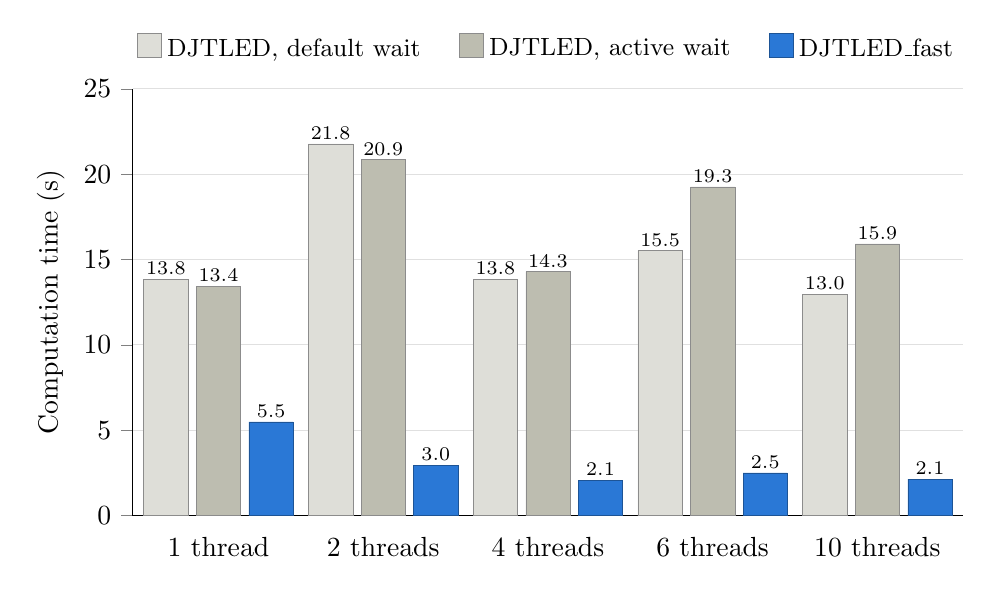
\begin{tikzpicture}
\begin{axis}[
  ybar=3pt, bar width=16pt,
  width=\linewidth, height=7cm,
  ymin=0, ymax=25,
  symbolic x coords={1,2,4,6,10}, xtick=data,
  xticklabels={1 thread,2 threads,4 threads,6 threads,10 threads},
  enlarge x limits=0.13,
  ylabel={Computation time (s)},
  ymajorgrids, grid style={black!12},
  axis lines*=left, tick align=outside, xtick style={draw=none},
  nodes near coords={\pgfmathprintnumber[fixed,fixed zerofill,precision=1]{\pgfplotspointmeta}},
  nodes near coords style={font=\scriptsize, text=black, inner sep=1.5pt},
  legend style={at={(0.5,1.04)}, anchor=south, legend columns=3, draw=none, font=\small,
                /tikz/every even column/.append style={column sep=1.2em}},
  legend image code/.code={\fill[#1] (0cm,-0.1cm) rectangle (0.3cm,0.2cm);},
]
\addplot[fill=refdefault, draw=black!45, line width=0.2pt] coordinates {(1,13.84) (2,21.77) (4,13.84) (6,15.52) (10,12.97)};
\addplot[fill=refactive, draw=black!45, line width=0.2pt] coordinates {(1,13.44) (2,20.86) (4,14.29) (6,19.26) (10,15.91)};
\addplot[fill=fastblue, draw=fastblue!70!black, line width=0.2pt] coordinates {(1,5.48) (2,2.95) (4,2.08) (6,2.50) (10,2.13)};
\legend{{DJTLED, default wait},{DJTLED, active wait},{\DJF}}
\end{axis}
\end{tikzpicture}
\caption{Large model: computation time in seconds for 2,001 steps of the 361,175-element model. Lower is better. Median of 2 runs per configuration on an Apple M5 with 4 performance and 6 efficiency cores. Threads do not speed up the reference; \DJF{} is up to 7 times faster.}
\label{fig:large}
\end{figure}

The reference takes about the same time with one, four and ten threads, and is slower with two. \DJF{} needs 5.5\,s on one thread and 2.1\,s on four. The speed-up over the faster reference configuration is 2.5 on one thread and between 6.1 and 7.1 on two to ten threads.

The single-thread figures isolate what the compact data layout and the cheaper arithmetic of Sections~\ref{sec:blocks} to~\ref{sec:newton} achieve without any parallelism: a factor of 2.1 on the small model and 2.5 on the large one. The rest of the gain on the large model comes from parallel scaling, which the reference does not have there. The likely cause is its strided distribution of elements (Section~\ref{sec:threads}): neighbouring 48-byte force records are written by different threads, so the threads continually invalidate each other's 64-byte cache lines. This explanation is consistent with the measurements but was not tested separately.

\DJF{} scales by a factor of 2.6 from one to four threads and gains nothing from the efficiency cores, which indicates that it is limited by memory bandwidth on this model.

\textbf{Complete run of the large model.} One complete run of 40,000 steps at four threads took 325.6\,s with the reference, or 8.1\,ms per step. \DJF{} took 62.9\,s when it was run immediately afterwards, on a machine already warmed by the reference run, and 45.4\,s in a separate run that started from a cool machine. The factor is therefore between 5.2 and 7.2. Per step, the complete runs are about 10 to 50\,\% slower than the short timed segment, because this fanless machine slows down as it warms up during a long run.

\subsection{Contribution of each change}
\label{sec:contrib}

Spin waiting and SIMD evaluation matter most on the small model; renumbering and SIMD evaluation matter most on the large one. Table~\ref{tab:contrib} gives the time of \DJF{} at four threads with one change removed at a time, and how much slower that is than with all changes.

\begin{table}[ht]
\centering
\small
\caption{\DJF{} at four threads with one change removed at a time. Small model: complete run. Large model: first 2,001 steps.}
\label{tab:contrib}
\begin{tabular}{@{}lrrrr@{}}
\toprule
Variant & Small model, ms & Slower by & Large model, s & Slower by \\
\midrule
All changes ($W = 8$) & 78 & & 2.04 & \\
Scalar kernel, $W = 1$ & 113 & 45\,\% & 2.76 & 35\,\% \\
Block width $W = 4$ & 91 & 17\,\% & 2.19 & 7\,\% \\
Block width $W = 16$ & 76 & $-3$\,\% & 2.06 & 1\,\% \\
\code{powf} instead of the warm-started iteration & 102 & 31\,\% & 2.32 & 14\,\% \\
No spin waiting & 140 & 79\,\% & 2.09 & 2\,\% \\
A parallel region per step & 79 & 1\,\% & 2.20 & 8\,\% \\
No renumbering & 95 & 22\,\% & 2.61 & 28\,\% \\
\bottomrule
\end{tabular}
\end{table}

Three points follow from Table~\ref{tab:contrib}.
\begin{itemize}
\item \textbf{The two models are limited by different things.} A step of the small model takes about 20 microseconds, so thread synchronisation and arithmetic dominate. A step of the large model takes about 1\,ms and moves far more data than fits in cache, so the order in which memory is visited dominates.
\item \textbf{A block width of eight is sufficient.} Widths of 8 and 16 are equal within the measurement spread, and a width of 4 is slower on both models.
\item \textbf{The persistent thread team contributes little on this runtime.} Its effect is 1\,\% on the small model. The two large-model runs of that variant differed by 13\,\%, so its 8\,\% there is uncertain.
\end{itemize}
The compact element record of Section~\ref{sec:blocks} cannot be switched off separately, because the whole solver is built on it. Its contribution is contained in the single-thread speed-ups of Section~\ref{sec:speed}.

\textbf{A caution on spin waiting.} Spin waiting assumes that every thread has a core to itself. During this work the small model was once run with ten threads while another program occupied the machine. The run took between 5 and 11\,s instead of 0.09\,s. On a shared or busy machine the passive wait policy should be used.

\subsection{Accuracy}
\label{sec:accuracy}

The two solvers agree to within 0.0016\,\% of the prescribed displacement on the small model and 0.042\,\% on the large one, and each is as close to the reference result as the other.

\textbf{Final displacement field.} Table~\ref{tab:accuracy} compares the nodal displacements at the end of the run. The difference at a node is the length of the difference vector. It is given in the length unit of the model and as a percentage of the prescribed displacement of 0.05.

\begin{table}[ht]
\centering
\small
\caption{Differences between final displacement fields. Percentages are relative to the prescribed displacement of 0.05.}
\label{tab:accuracy}
\begin{tabular}{@{}llrrrr@{}}
\toprule
Model & Comparison & Largest difference & Largest, \% & RMSE & RMSE, \% \\
\midrule
Small & DJTLED vs reference & $7.41\times10^{-7}$ & 0.0015 & $2.07\times10^{-7}$ & 0.0004 \\
Small & \DJF{} vs reference & $8.51\times10^{-7}$ & 0.0017 & $2.29\times10^{-7}$ & 0.0005 \\
Small & \DJF{} vs DJTLED & $8.12\times10^{-7}$ & 0.0016 & $2.11\times10^{-7}$ & 0.0004 \\
\addlinespace
Large & DJTLED vs reference & $2.54\times10^{-5}$ & 0.051 & $4.52\times10^{-6}$ & 0.0090 \\
Large & \DJF{} vs reference & $2.15\times10^{-5}$ & 0.043 & $4.54\times10^{-6}$ & 0.0091 \\
Large & \DJF{} vs DJTLED & $2.11\times10^{-5}$ & 0.042 & $4.01\times10^{-6}$ & 0.0080 \\
\bottomrule
\end{tabular}
\end{table}

On both models the difference between the two solvers is the same size as the distance of either solver from the reference. The changes of Section~\ref{sec:method} therefore add no error that can be distinguished from the rounding already present in the reference implementation. On the small model the differences are close to the six significant digits with which the displacements are written to file.

\textbf{Independence of the CPU configuration.} For each solver, the output files of the small model are byte-for-byte identical with 1, 2, 4 and 10 threads. For \DJF{} they are also identical for SIMD widths of 1, 4, 8 and 16, with and without the persistent thread team, and with and without spin waiting. This follows from the fixed summation order of Section~\ref{sec:unchanged}. The accuracy figures above therefore hold for every CPU configuration in Section~\ref{sec:speed}.

\textbf{Warm start.} The Newton iteration of Section~\ref{sec:newton} never needed its \code{powf} fallback: zero fallbacks in $2.7\times10^{7}$ element evaluations on the small model and in $1.4\times10^{10}$ on the large one.

\textbf{Why the large model shows larger differences.} The differences are about 30 times larger on the large model. Three properties of the model point to single-precision rounding as the cause. It runs ten times as many steps, and each adds a rounding error. Its time step is ten times smaller, so the displacement increment of a step is smaller relative to the displacement it is added to. Its elements are smaller, so the deformation of an element is the difference of nearly equal nodal displacements.

\textbf{Sensitivity to the time step.} A sweep of the time step on the large model supports this reading. \DJF{} was run with 16 time steps between 0.00002 and 0.000045 (Figure~\ref{fig:sweep}).

\begin{figure}[ht]
\centering
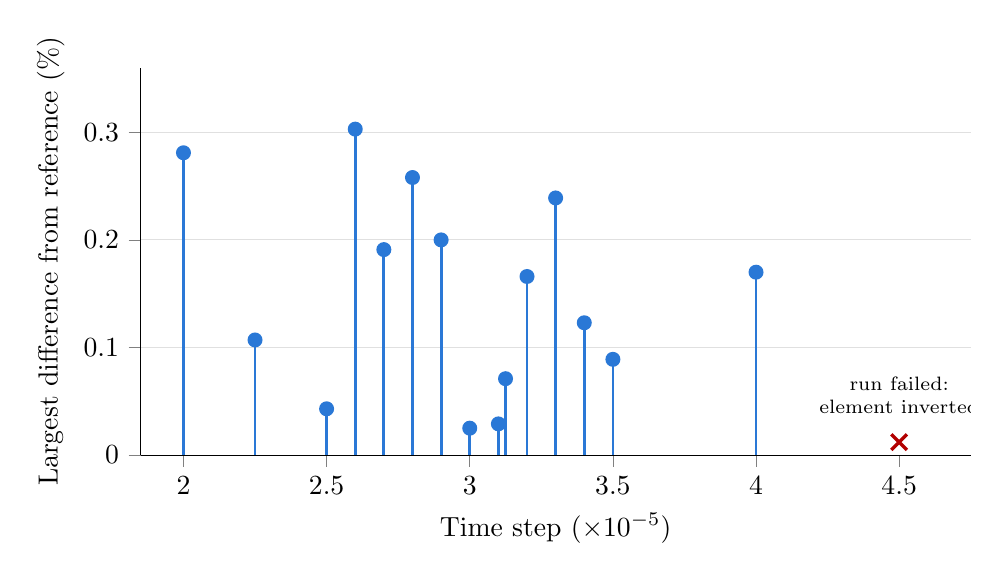
\begin{tikzpicture}
\begin{axis}[
  width=\linewidth, height=6.5cm,
  xmin=1.85, xmax=4.75, ymin=0, ymax=0.36,
  xlabel={Time step ($\times10^{-5}$)},
  ylabel={Largest difference from reference (\%)},
  ymajorgrids, grid style={black!12},
  axis lines*=left, tick align=outside,
  xtick={2,2.5,3,3.5,4,4.5},
  ytick={0,0.1,0.2,0.3},
  yticklabel style={/pgf/number format/fixed, /pgf/number format/precision=1},
  xticklabel style={/pgf/number format/fixed, /pgf/number format/precision=1},
]
\addplot[ycomb, color=fastblue, line width=1pt, mark=*, mark size=2.2pt, mark options={fill=fastblue}] coordinates {
  (2.0,0.281) (2.25,0.107) (2.5,0.043) (2.6,0.303) (2.7,0.191) (2.8,0.258) (2.9,0.200)
  (3.0,0.025) (3.1,0.029) (3.125,0.071) (3.2,0.166) (3.3,0.239) (3.4,0.123) (3.5,0.089) (4.0,0.170)};
\addplot[only marks, mark=x, mark size=4pt, color=red!70!black, line width=1.2pt] coordinates {(4.5,0.012)};
\node[anchor=south, font=\scriptsize, align=center] at (axis cs:4.5,0.03) {run failed:\\element inverted};
\end{axis}
\end{tikzpicture}
\caption{Large model: largest nodal difference from the reference result, as a percentage of the prescribed displacement, for 16 complete runs of \DJF{} at 4 threads with different time steps. The difference does not decrease as the step is reduced.}
\label{fig:sweep}
\end{figure}

The difference from the reference varies between 0.025\,\% and 0.30\,\% and does not decrease as the step is reduced. Neighbouring steps can differ by a factor of eight. A time-discretisation error would shrink smoothly with the step, so this scatter is rounding noise. Two practical consequences follow. First, on a model of this size, differences below about 0.3\,\% between two single-precision runs are not evidence of an error in either. Second, the time step should be chosen for stability, not for agreement with a reference.

\textbf{Stability limit.} The run with a step of 0.000045 failed when an element inverted at step 20,041 of 22,223, and the step of 0.00005 supplied with the model failed in both solvers. Steps of 0.00004 and below were stable. The bound of Eq.~\eqref{eq:stability}, evaluated with the shortest element altitude of 0.348\,mm and a wave speed of 17.8\,m/s, gives 0.0000196. The observed limit is about twice that estimate. All results for the large model in this paper use a step of 0.000025, which divides the total time into exactly 40,000 steps.

%======================================================================
\section{Conclusion}
\label{sec:conclusion}

\DJF{} computes the same DJ-TLED solution as the reference implementation 2.1 to 2.7 times faster on a 6,713-element model and up to 7 times faster on a 361,175-element model, with no loss of accuracy that can be measured against the reference.

\textbf{Where the gain comes from.} The compact element record, the simplified force expression and the warm-started iteration for $\Jm$ make one thread 2.1 to 2.5 times faster. On the large model the remaining factor comes from parallel scaling: \DJF{} is 2.6 times faster on four threads than on one, whereas the reference is no faster on four or ten threads than on one. Among the individual changes, spin waiting and SIMD evaluation matter most for the small model, and renumbering and SIMD evaluation for the large one.

\textbf{Accuracy.} The two solvers differ by 0.0016\,\% of the prescribed displacement on the small model and 0.042\,\% on the large one. In both cases this equals the distance of either solver from the reference result. The results of each solver are identical for every thread count.

\textbf{Three findings beyond the speed-up.}
\begin{itemize}
\item \textbf{Run conditions change the conclusion.} The wait policy of the OpenMP runtime alone makes the reference 1.3 times faster on the small model. A comparison that grants this setting to only one solver overstates the speed-up, here as 3.2 instead of 2.4.
\item \textbf{Single precision limits what can be compared.} On the large model the final displacements move by up to 0.3\,\% of the prescribed displacement when only the time step is changed, with no trend. Agreement finer than that cannot be expected from either solver.
\item \textbf{The reference does not scale on a large mesh.} Its strided distribution of elements over threads is the likely cause.
\end{itemize}

\textbf{Limits of this study.} All measurements come from one machine, an Apple M5 without a fan. Both models are the same cube in tension with one material and one element type. The thread-scaling figures of the large model were timed on the first 2,001 steps. The cache-line explanation for the reference's lack of scaling was not tested in isolation. Other processors, operating systems and loading cases were not measured.

\textbf{Next steps.} The rounding scatter suggests carrying the displacement update in double precision while keeping the force kernel in single precision. Since the large model is limited by memory bandwidth, a smaller force buffer or a single pass per step would help more than further arithmetic savings. The block layout of Section~\ref{sec:blocks} is also the layout a GPU kernel needs, which makes it a natural basis for a GPU version.

%======================================================================
\begin{thebibliography}{9}

\bibitem{zhang2021}
Zhang J. A direct Jacobian total Lagrangian explicit dynamics finite element algorithm for real-time simulation of hyperelastic materials. \emph{International Journal for Numerical Methods in Engineering}. 2021;122(20):5744--5772. \href{https://doi.org/10.1002/nme.6772}{doi:10.1002/nme.6772}. Preprint: \href{https://arxiv.org/abs/2106.14189}{arXiv:2106.14189}.

\bibitem{miller2007}
Miller K, Joldes G, Lance D, Wittek A. Total Lagrangian explicit dynamics finite element algorithm for computing soft tissue deformation. \emph{Communications in Numerical Methods in Engineering}. 2007;23(2):121--134. \href{https://doi.org/10.1002/cnm.887}{doi:10.1002/cnm.887}.

\bibitem{taylor2008}
Taylor ZA, Cheng M, Ourselin S. High-speed nonlinear finite element analysis for surgical simulation using graphics processing units. \emph{IEEE Transactions on Medical Imaging}. 2008;27(5):650--663. \href{https://doi.org/10.1109/TMI.2007.913112}{doi:10.1109/TMI.2007.913112}.

\bibitem{djtledcode}
Zhang J. DJTLED: source code of the reference implementation. \href{https://github.com/jinaojakezhang/DJTLED}{github.com/jinaojakezhang/DJTLED}.

\bibitem{cuthill1969}
Cuthill E, McKee J. Reducing the bandwidth of sparse symmetric matrices. In: \emph{Proceedings of the 1969 24th National Conference of the ACM}. 1969:157--172. \href{https://doi.org/10.1145/800195.805928}{doi:10.1145/800195.805928}.

\end{thebibliography}

\end{document}
